\documentclass[10pt]{article}

% Für Demonstrationszwecke
\usepackage{lipsum}



%\usepackage{titling}
\usepackage[utf8]{inputenc}
\usepackage[ngerman]{babel}
\usepackage{scrpage2}
\usepackage{graphicx}
%\usepackage{lastpage}
%\usepackage[a4paper,left=2.5cm,right=2cm,top=1cm,bottom=2.5cm]{geometry}
\usepackage{float}
\usepackage[scaled]{uarial}
%\renewcommand*\familydefault{\sfdefault} 
\usepackage[T1]{fontenc}
%\usepackage{booktabs}
%\usepackage{pdflscape}
\usepackage[table,xcdraw]{xcolor}

\renewcommand{\headfont}{}

\usepackage{hyperref}
\usepackage{glossaries}
\input{glossary}


\usepackage[square,numbers]{natbib} 
\bibliographystyle{plainnat}

\title{Software Requirement Specification}
\date{06.10.2016}
\author{\textbf{ESE Team 9} \\ \\Sven Kellenberger\\Rapfael
Ottersbach\\Levi Ryffel\\Marcel Schmutz\\Kevin Studer}




%\pagestyle{scrheadings}
%\ihead{Test}
%\ohead{Test}
%\ofoot{Test}



\begin{document}
\maketitle
\pagebreak
\tableofcontents
\pagebreak

\section{Introduction}

\subsection{Purpose}
This document presents a detailed description of the web application Flatfindr.
Foremost, it provides a legaly binding contract between the stakeholders and the
developer team 9. This document is a RUP conform SRS document.

\subsection{Scope of the Project}
The web application Flatfindr will help the participating user to promote free
places in their rooms or flats. Also it should help user to search for free
places in rooms or flats.

More specifically, the application will provide methods to search for free
flats, help to ensure flats with specific parameters are presented for users and
that the application will provide enough methods, to get in contact with the
advertiser. On the other side, users will be able to insert an ad for a free
place in their flats, will help define the visitation time (if an user wants to
see the flat which is advertised) and provide some other instruments to describe
the flat as best as possible.

\subsection{Glossary}

\begin{table}[H]
	\centering
	\begin{tabular}{p{3cm}p{9cm}}
	\multicolumn{1}{c}{\textbf{Term}} & \multicolumn{1}{c}{\textbf{Description}} \\
Advertiser & User who advertise his free place in his room or flat. \\
RUP & Stands for Rational Unified Process. Process developed by IBM. Has the SRS document as a requirement for all development activities. \\
SRS & Stands for Software Requirements Specification. A document that completely describes all of the functions of a proposed system and the constraints under which it must operate. \\
Stakeholder & Any person with an interest in the project who is not a developer. \\
User & Participant in the application. Can either be a normal user who searches for a flat or an advertiser. 
	\end{tabular}
	\caption{Glossary}
	\label{table-glossary}
\end{table}

\subsection{Stakeholders}
The table \ref{table-stakeholders} will give an overview of the known
Stakeholders.
\begin{table}[H]
	\centering
	\begin{tabular}{ll}
	\multicolumn{1}{c}{\textbf{Name}} & \multicolumn{1}{c}{\textbf{Contact}} \\
	ESE Assistant & ?                                        
	\end{tabular}
	\caption{Stakeholders}
	\label{table-stakeholders}
\end{table}
%TODO: Identify Stakeholders

\subsection{System Overview}
The image \ref{image-system-overview} will introduce a general system overview
of the product in development.
\begin{figure}[p]
    \centering
	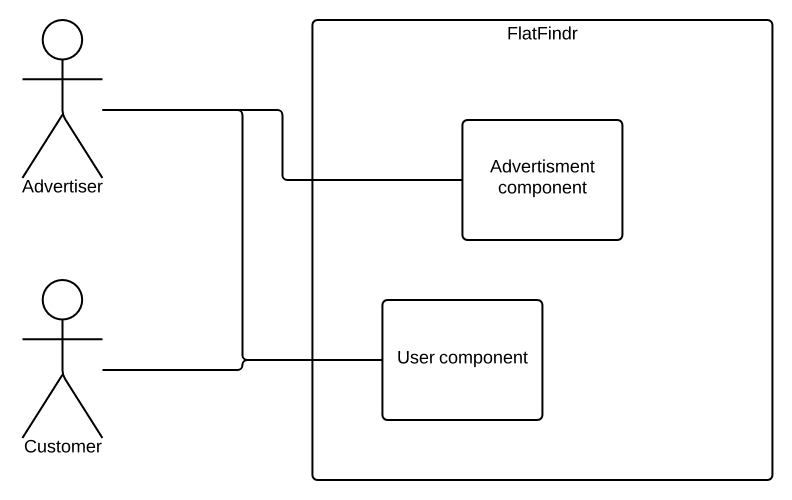
\includegraphics[width=12cm]{images/system-overview}
	\caption{System Overview}
    \label{image-system-overview}
\end{figure}

\subsection{References}

\section{Overall Description}
\section{External Interfaces}

\subsection{User Interfaces}
	As is shown by image \ref{image-flatfindrScreenshot}, the user interface is
	straight forward due to it being a homepage.
	
\begin{figure}[p]
    \centering
	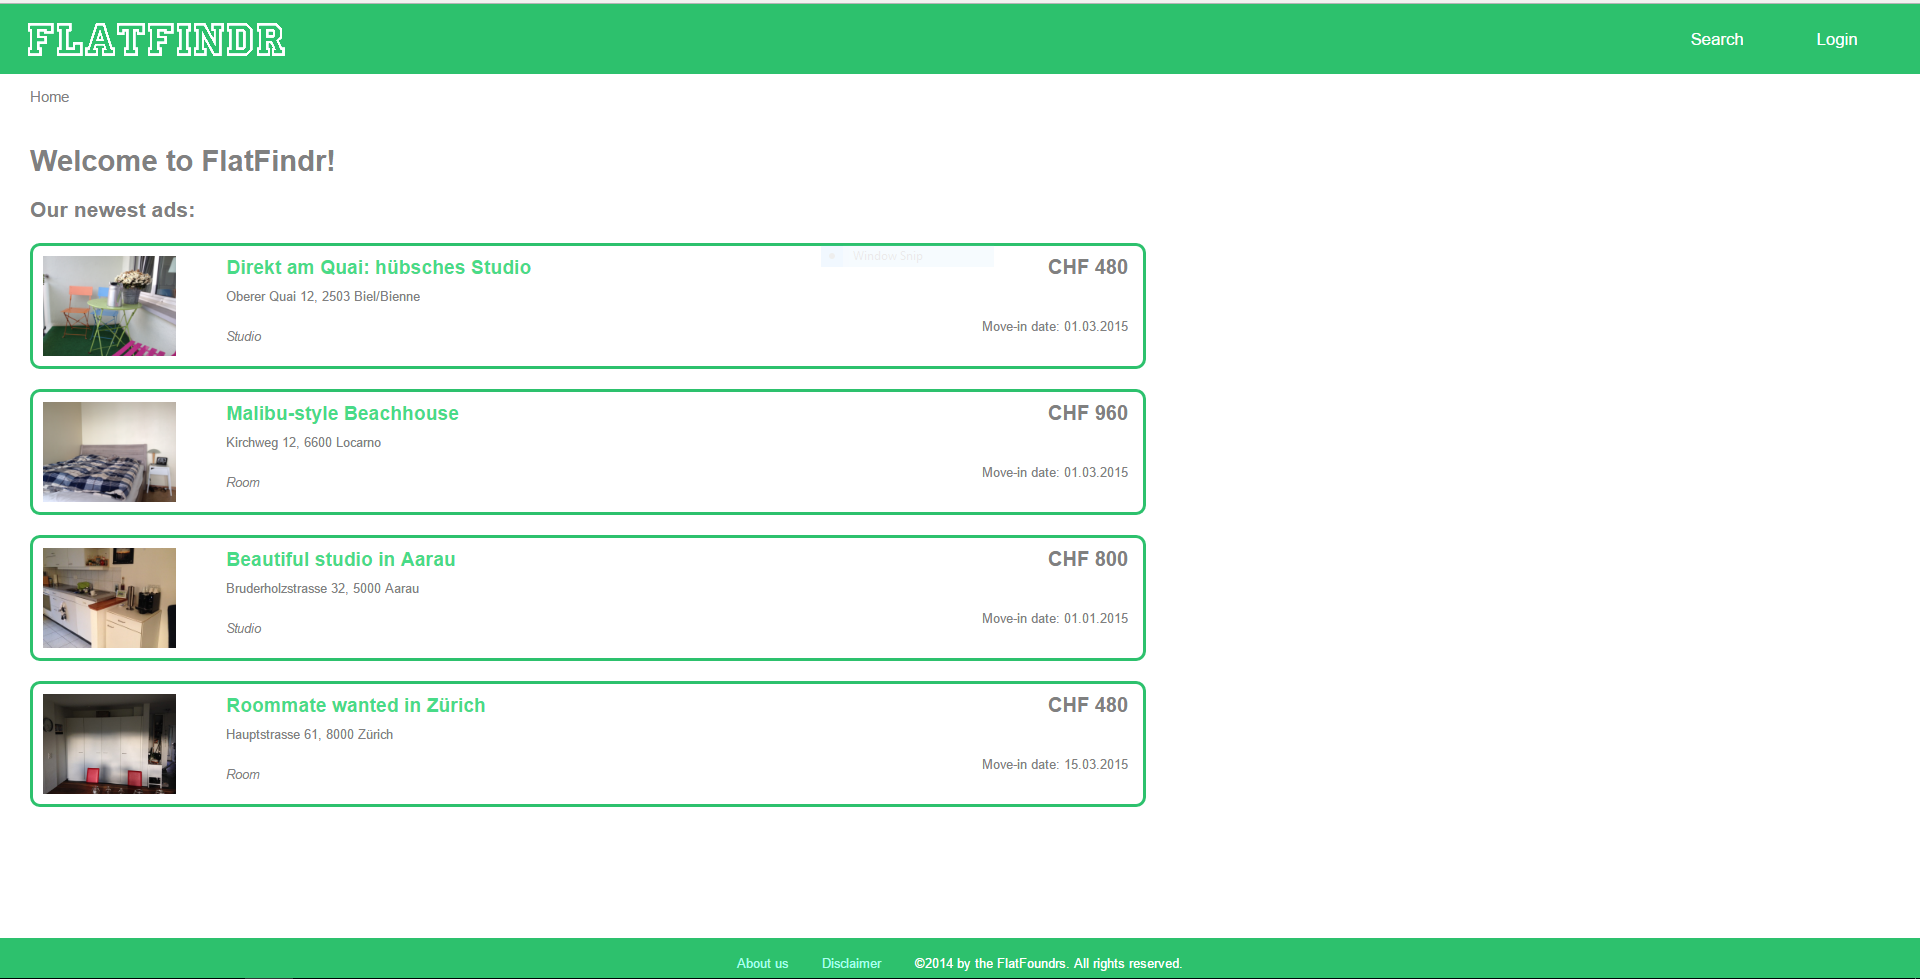
\includegraphics[width=12cm]{images/flatfindrScreenshot}
	\caption{GUI}
    \label{image-flatfindrScreenshot}
\end{figure}
	
\subsection{Hardware Interfaces}
	The homepage will be able to be displayed on a computer, as well as mobile
	phones and tablets.
	

\section{System Features}

\subsection{Use-Cases}

\begin{table}[H]
\centering
\label{table-use-case-1}
\begin{tabular}{|p{3cm}|p{10cm}}
Use Case ID       & 1                                                                                                                                                              \\
Use Case Name     & Login                                                                                                                                                          \\
Trigger           & A user wants to login to the webapplication                                                                                                                   \\
Precondition      & The user has already an account on the webapplication                                                                                                          \\
Basic Path        & \begin{enumerate}
\item The user access the webapplication and selects the link "Login"
\item The user enters his credentials for his account
\item The user is redirected to the homepage
\end{enumerate} 
     \\
Alternative Paths & None                          \\
Postconditions    & The user is logged-in                                                                                                                                          \\
Exception Paths   & In step 2, if the user enters not valid credentials into the system, the system should exit with the error message, that the credentials were wrong            \\
Other             & n/a                                                                                                                                                                                                        
\end{tabular}
\caption{Use Case 1}
\end{table}

\begin{table}[H]
\centering
\label{table-use-case-2}
\begin{tabular}{|p{3cm}|p{10cm}}
Use Case ID       & 2                                                         \\
Use Case Name     & Post ad to sell property                                \\
Trigger           & A user wants to sell a property					\\
Precondition      & The user is logged in\\
Basic Path        & \begin{enumerate}
\item The user accesses the webapplication and selects the link 'Sell'
\item The user is redirected to a form, where he can enter the information
about the property he wants to sell. He can also add pictures and among other
options he can select wheter he wants to sell directly or through an auction. 
\item After submitting the form the user is redirected to the finished page of
his ad
\end{enumerate} 
     \\
Alternative Paths & None                          \\
Postconditions    & The user has the new ad attached to his account.                                                          
\\
Exception Paths   & None            \\
Other             & n/a                                                                                                                                                                                                        
\end{tabular}
\caption{Use Case 2}
\end{table}

\begin{table}[H]
\centering
\label{table-use-case-3}
\begin{tabular}{|p{3cm}|p{10cm}}
Use Case ID       & 3                                                           \\
Use Case Name     & Buy property directly                                                         \\
Trigger           & A user wants buy the property described in an ad he saw directly \\
Precondition      & The user is logged in and on the ad page of the property he wants to buy\\
Basic Path        & \begin{enumerate}
\item The user selects the link 'Buy'
\item The user is redirected to a page with a form through which he can contact the seller
\item After submitting the message and the contact data of the buyer is forwarded to the seller and the user is redirected to the ad page
\end{enumerate} 
     \\
Alternative Paths & None                          \\
Postconditions    & None				\\
Exception Paths   & None            \\
Other             & n/a                                                                                                                                                                                                        
\end{tabular}
\caption{Use Case 3}
\end{table}

\begin{table}[H]
\centering
\label{table-use-case-4}
\begin{tabular}{|p{3cm}|p{10cm}}
Use Case ID       & 4                                                         \\
Use Case Name     & Bid on a property                                                          \\
Trigger           & A user wants to bid on the auction of a property                                          \\
Precondition      & The user is logged in and on the auction page                                                  \\
Basic Path        & \begin{enumerate}
\item The user selects the specific auction he wants to participate in
\item The user is redirected to the auction page, where information about the
property and the auction itself (current bid, amount of bidders, time until
the deadline etc.) is displayed
\item The user can enter a bid of his own which has to be higher than the
present highest bid. 
\end{enumerate} 
     \\
Alternative Paths & None                          \\
Postconditions    & The highest bid now displays the bid made by the user                                                       \\
Exception Paths   & In step 3 if the bid is not higher than the present one an error flashes to point the fact out.					\\
Other             & n/a                                                                                                                                                                                                        
\end{tabular}
\caption{Use Case 4}
\end{table}

\begin{table}[H]
\centering
\label{table-use-case-5}
\begin{tabular}{|p{3cm}|p{10cm}}
Use Case ID       & 5                                                         \\
Use Case Name     & Search for porperties on sale                                                         \\
Trigger           & A user wants to look for properties on sale                                         \\
Precondition      & The user is logged in and on the search page                             \\
Basic Path        & \begin{enumerate}
\item The user selects in the search criterias that he wants to look for
properties on sale
\item All properties on sale (directly or through an auction) matching his other
search criterias are displayed to the user
\end{enumerate} 
     \\
Alternative Paths & None                          \\
Postconditions    & None                                                      \\
Exception Paths   & None				\\
Other             & n/a                                                                                                                                                                                                        
\end{tabular}
\caption{Use Case 5}
\end{table}

\begin{table}[H]
\centering
\label{table-use-case-6}
\begin{tabular}{|p{3cm}|p{10cm}}
Use Case ID       & 6                                                         \\
Use Case Name     & Create a search alert                                                         \\
Trigger           & A user wants to create a search alert                                         \\
Precondition      & The user is logged in and on the search page                          \\
Basic Path        & \begin{enumerate}
\item The user selects the link 'Create search alert'
\item The user is redirected to a form where he can select the search criterias
he want to cover with his alert
\item After submitting the form the user is redirected to the search page 
\end{enumerate} 
     \\
Alternative Paths & None                          \\
Postconditions    & The search alert is attached to the profile of the user and
he gets an email notification every time a new ad for a property matching his
alert criterias is created			\\
Exception Paths   & None				\\
Other             & n/a                                                                                                                                                                                                        
\end{tabular}
\caption{Use Case 6}
\end{table}

\begin{table}[H]
\centering
\label{table-use-case-7}
\begin{tabular}{|p{3cm}|p{10cm}}
Use Case ID       & 7                                                         \\
Use Case Name     & Delete or disable a search alert                                      \\
Trigger           & A user wants to delete or disable a previously created search alert	\\
Precondition      & The user is logged in and on his profile page               \\
Basic Path        & \begin{enumerate}
\item The user selects the link 'Search Alerts'
\item The user is redirected to the search alerts page, where all his search
alerts are displayed. He can now delete or disable each search alert via the
respective buttons. 
\end{enumerate} 
     \\
Alternative Paths & None                          \\
Postconditions    & The user gets no longer notifications for disabled or deleted search alerts		\\
Exception Paths   & None			\\
Other             & n/a                                                                                                                                                                                                        
\end{tabular}
\caption{Use Case 7}
\end{table}
\section{Other Requirements}



%\section{Abstract}

%\pagebreak
%\appendix

%\section{Glossar}

%\renewcommand{\glossarysection}[2][]{}
%\printglossaries



% \section{Referenzen}

% \begingroup
% \renewcommand{\section}[2]{}
% \bibliography{../../Zitatsammlung/Allgemein}
% \endgroup

\end{document}